\section{Accuracy}
\label{sec:accuracy}

Each error figure names its reference (M mesh, T continuum, P point). The three
references stay apart throughout:
the mesh $M$, the TSC-convolved continuum $T$ (Eq.~\eqref{eq:Fc}, the
quantity the mesh is built to compute), and the point field $P$ (the
un-smoothed Li\'enard--Wiechert field). $M$ against $T$ is the discrete
deposit and convolution error. $T$ against $P$ is the TSC smoothing, an
$O(1)$ effect at $\gamma h \gg 1$. $M$ against $P$ is the total.

\subsection{The reference and the two metrics}

The arbiter is an independent TSC-convolved continuum, a tensor
Gauss--Legendre quadrature with a TSC-knot split and a singularity-cancelling
power map \citep{indfield}. Its quadrature error is below the
$3\times10^{-4}$ gate in every configuration measured here \citep{N2b}.

Two metrics are reported and are not interchangeable. The judge metric
$|\mathrm{ref}-\mathrm{mesh}|/(1+\max(|\mathrm{ref}|,\mathrm{mesh}|))$ is
absolute-dominated: for fields of order $10^{-9}$ V/m the $+1$ denominator
swamps the error, so it reports a crossover at $d=2$ for every case and does
not discriminate \citep{W4b}. The relative per-component error
$|\mathrm{ref}-\mathrm{mesh}|/\max(|\mathrm{ref}|,\mathrm{mesh}|)$, over
components where $|\mathrm{ref}|\ge10^{-3}$ of the local field, is the
meaningful one. This section reports relative error as the metric of record.

\subsection{Reference-separated error at $d=48$}

\begin{table}[t]
\centering
\small
\caption{L2-pooled relative error at $d=48$ cells, $h=1$, perpendicular
direction (L2 over the six components; the single-component worst for
$\gamma=1$, aspect 4, $M\!-\!T$ is $2.65\times10^{-5}$ and for
$\gamma=10$, aspect 1 is $1.4\times10^{-3}$) \citep{N2b}.
$M\!-\!T$: mesh vs TSC-convolved continuum (the target). $M\!-\!P$: mesh vs
point field. $T\!-\!P$: TSC smoothing, mesh-independent. At $\gamma=10$,
aspect 1, the gap between $M\!-\!P$ and $M\!-\!T$ is the smoothing
($1.5\times10^{-2}$ vs $2.6\times10^{-4}$, an L2 ratio of $58\times$), not
the mesh.}
\label{tab:d48}
\begin{tabular}{lrrrr}
\toprule
$\gamma$ & aspect & $M\!-\!T$ & $M\!-\!P$ & $T\!-\!P$ \\
\midrule
1   & 1 & $1.38\times10^{-7}$ & $9.89\times10^{-8}$ & $3.96\times10^{-8}$ \\
1   & 4 & $2.65\times10^{-5}$  & $2.39\times10^{-3}$  & $2.40\times10^{-3}$  \\
10  & 1 & $2.6\times10^{-4}$    & $1.5\times10^{-2}$   & $1.48\times10^{-2}$  \\
10  & 4 & $3.33\times10^{-2}$  & $1.19\times10^{-1}$  & $1.44\times10^{-1}$  \\
100 & 1 & $3.75\times10^{-1}$  & $2.20\times10^{-1}$  & $4.40\times10^{-1}$  \\
100 & 4 & $2.78\times10^{0}$   & $2.49\times10^{-1}$  & $8.32\times10^{-1}$  \\
\bottomrule
\end{tabular}
\end{table}

Table~\ref{tab:d48} shows two things. At $\gamma=10$, aspect 1, the mesh
against the point field ($M\!-\!P=1.5\times10^{-2}$) is about $58\times$ the
mesh against its own target ($M\!-\!T=2.6\times10^{-4}$, an L2 ratio); the
difference is
the TSC smoothing, which $M\!-\!P$ inherits and $M\!-\!T$ does not. A
mesh-versus-point comparison measures the shape the deposit applies, not the
discretization error. Second, the $M\!-\!T$ error is not converged
perpendicular to the beam at $\gamma h \gg 1$: at aspect 1 it is acceptable
only for $\gamma=10$ and not for $\gamma=100$; at aspect 4 it is not
converged at any $\gamma$. Only the axial direction is clean at every
$\gamma$ \citep{N2b}.

\subsection{The independent validation}

A second, independent pass measured the shipped CLI end to end:
\texttt{picBunch} at \texttt{bfaa1e26} (field path unchanged through
v0.1.3), rosi\_v100, \texttt{indfield.py}
order $12$ refine $3$, $d=2$ to $32$ cells, $\gamma\in\{1,10\}$, aspect 1
and 4, single particle and three-particle cloud \citep{W4b}.

\begin{table}[t]
\centering
\small
\caption{Worst per-component relative error (over $x,y$, $|\mathrm{ref}|
\ge10^{-3}$ of the local field) of the shipped CLI against the
TSC-convolved continuum, at $d=16$ and $d=32$ cells; rosi\_v100,
\texttt{indfield.py} order $12$ refine $3$ \citep{W4b}. ``s/c'' = single /
cloud. $\gamma=10$ does not cross $3\times10^{-4}$ within $32$ cells;
$\gamma=1$ crosses at $d=12$ (aspect 1) and $d=32$ (aspect 4).}
\label{tab:w4b}
\begin{tabular}{llrr}
\toprule
$\gamma$, aspect & s/c & $d\!=\!16$ & $d\!=\!32$ \\
\midrule
1, 1  & $3.5\mathrm{e}{-5}$ / $1.0\mathrm{e}{-4}$ & $2.2\mathrm{e}{-6}$ / $2.0\mathrm{e}{-5}$ \\
1, 4  & $2.8\mathrm{e}{-3}$ / $2.1\mathrm{e}{-3}$ & $2.0\mathrm{e}{-4}$ / $2.6\mathrm{e}{-4}$ \\
10, 1 & $5.6\mathrm{e}{-2}$ / $5.3\mathrm{e}{-2}$ & $6.3\mathrm{e}{-3}$ / $6.5\mathrm{e}{-3}$ \\
10, 4 & $5.5\mathrm{e}{-2}$ / $5.0\mathrm{e}{-2}$ & $6.3\mathrm{e}{-3}$ / $6.4\mathrm{e}{-3}$ \\
\bottomrule
\end{tabular}
\end{table}

Table~\ref{tab:w4b} confirms the reference-separated picture independently.
$\gamma=1$ crosses $3\times10^{-4}$ at $d=12$ (aspect 1, $1.1\times10^{-4}$)
and $d=32$ (aspect 4, $2.6\times10^{-4}$); at $\gamma=10$ the relative error
floors near $6\times10^{-3}$ at $d=32$ for all four cases and does not cross
$3\times10^{-4}$ within the swept range. The near shell is far worse, with
relative error $O(0.4)$--$0.8$ at $d=2$. The window starts at $d=2$, so the
TSC support interior ($|s|<1.5$ cells) is not covered \citep{W4b}.

\begin{figure}[t]
\centering
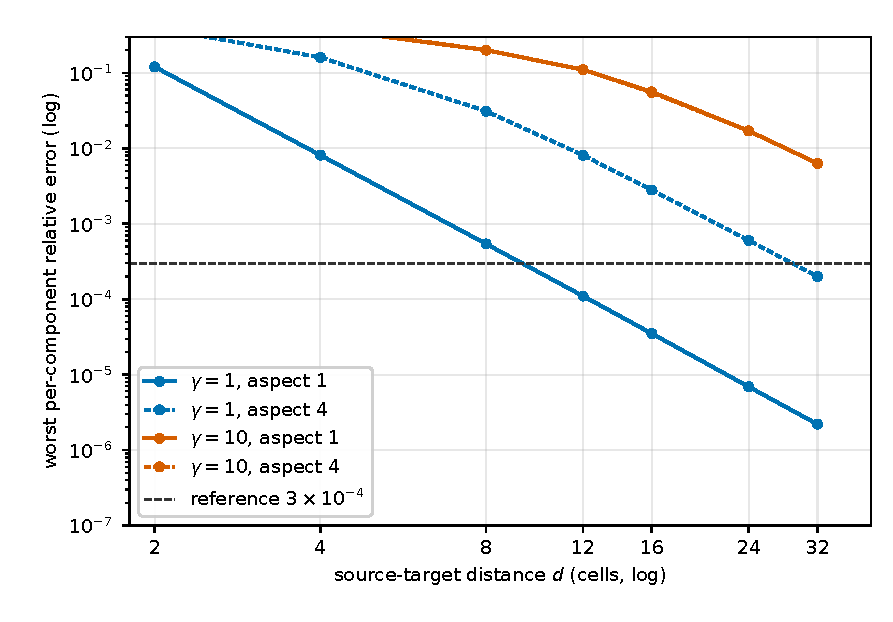
\includegraphics[width=0.95\linewidth]{figs/F_w4b_rel_error.pdf}
\caption{Worst per-component relative error of the shipped CLI against the
TSC-convolved continuum, per $d$ in cells, single-particle series only (the
three-particle cloud is in Table~\ref{tab:w4b}); rosi\_v100,
\texttt{indfield.py}
order $12$ refine $3$ \citep{W4b}. Solid, $\gamma=1$; dashed, $\gamma=10$;
blue, aspect 1; orange, aspect 4. $\gamma=1$ crosses the $3\!\cdot\!10^{-4}$
gate at $d=12$ (aspect 1) and $d=32$ (aspect 4); $\gamma=10$ floors near
$6\!\cdot\!10^{-3}$ at $d=32$ and never crosses within the swept range.}
\label{fig:Fw4b}
\end{figure}

The point-field column (Table~\ref{tab:d48}, $M\!-\!P$) is the mesh against
the un-smoothed field. It carries the TSC smoothing in addition to the deposit
error, and the two never agree for $\gamma h \gg 1$. The first half's distance
sweep (Fig.~\ref{fig:Fw4b}) plots this point-field comparison; the
$M\!-\!T$ column of Table~\ref{tab:d48} is the mesh against its own target.

\subsection{Crossover radii}

\begin{table}[t]
\centering
\small
\caption{Crossover radius in cells: first $d$ at which every larger $d$ is at
or below the gate, $h=1$, L2 over the six components, per axis direction,
worst over the three positive axis directions ($>$48: not reached)
\citep{N2b}. $T$: TSC-convolved continuum; $P$: point field. Oblique
directions are $\sim1.5\times$ larger. The $\gamma=1$ aspect 1 row is $d=8$
against both references here, versus the $d=12$ of the shipped-CLI series in
Table~\ref{tab:w4b}: the two measurements use different component sets (six
axis directions, L2-pooled, versus the per-component relative error over
$x,y$) and different implementations (the N2b standalone measurement versus
the shipped executable), so they are not the same crossover
\citep{N2b,W4b}.}
\label{tab:crossover}
\begin{tabular}{lcc|cc|cc}
\toprule
 & \multicolumn{2}{c}{$3\!\times\!10^{-4}$} & \multicolumn{2}{c}{$10^{-3}$} \\
\cmidrule(lr){2-3}\cmidrule(lr){4-5}
$\gamma$ & aspect & ref & axial $z$ & perp $x$ & axial $z$ & perp $x$ \\
\midrule
1   & 1 & $T$ & 8  & 8  & 6  & 6  \\
    & 1 & $P$ & 8  & 8  & 6  & 6  \\
1   & 4 & $T$ & 6  & 24 & 6  & 16 \\
    & 4 & $P$ & 48 & $>48$ & 32 & $>48$ \\
10  & 1 & $T$ & 6  & 48 & 6  & 48 \\
    & 1 & $P$ & $>48$ & $>48$ & 32 & $>48$ \\
10  & 4 & $T$ & 6  & $>48$ & 6  & $>48$ \\
    & 4 & $P$ & $>48$ & $>48$ & 32 & $>48$ \\
100 & 1 & $T$ & 6  & $>48$ & 6  & $>48$ \\
    & 1 & $P$ & $>48$ & $>48$ & 32 & $>48$ \\
100 & 4 & $T$ & 6  & $>48$ & 6  & $>48$ \\
    & 4 & $P$ & $>48$ & $>48$ & 32 & $>48$ \\
\bottomrule
\end{tabular}
\end{table}

At $\gamma=1$, aspect 1, the mesh is within $3\times10^{-4}$ of both
references from $d=8$; the two are interchangeable there. From $\gamma=10$
up, against the point field the perpendicular direction does not reach
$3\times10^{-4}$ within $48$ cells; against the target the perpendicular
crossover is $48$ ($\gamma=10$, aspect 1) or not reached. The axial
direction stays at $6$ against the target at every $\gamma$ \citep{N2b}.

\subsection{The disagreement is per-source}

On a $64\times64\times32$, cell $10^{-7}$\,m, stationary bunch ($\gamma=1$),
the disagreement with the exact-quadrature reference does not grow with
particle count: outside the TSC support the worst per-component error stays
in the $10^{-3}$ to $3\times10^{-2}$ band across $N=1$ to $1000$
\citep{W7t}. The $O(1)$ values at $N\ge10$ occur only because the global
worst sample point falls $0.42$--$0.65$ cells from a source, inside that
source's TSC support. A flat per-source floor is what a kernel or
reference-type difference produces; a charge-weighting defect would grow with
$N$. The measured disagreement is the in-support, near-source regime, and it
does not depend on the number of sources \citep{W7t}.

\subsection{The $h^{3}$ defect and its correction}

Section~\ref{sec:method} derives the $h^{3}$ factor and the $1/h^{3}$
overshoot of the delivered mesh. Fig.~\ref{fig:Ff} is the measured
per-$h$ series, worst per-component relative error against
\texttt{indfield.py}, at fixed physical separation,
$\gamma\in\{1,10\}$, aspect 1 and 4, rosi\_v100. The per-$h$ runs are at
fixed physical separation, so they are not a scale-invariance demonstration
(Section~\ref{sec:scaleinvariance}); they show that the after-fix field is
stable to about $9\times10^{-4}$ over $h=1$ to $1/2$ (the refine gate,
below), while the pre-fix field, $1/h^{3}$ too large in absolute terms, has
a relative error that rises toward $1$ as $h$ is refined (only the absolute
error scales as $h^{-3}$; the relative error saturates because the
reference is not scaled with it) \citep{F4}.

\begin{figure}[t]
\centering
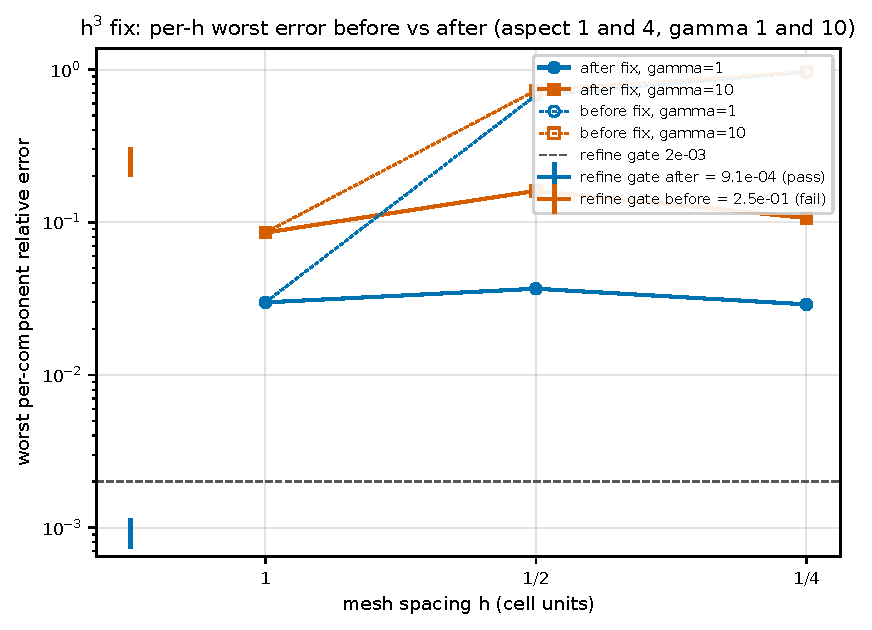
\includegraphics[width=0.95\linewidth]{figs/F_f_h3_regression.pdf}
\caption{Measured per-$h$ worst per-component relative error before and
after the $h^{3}$ fix (commit \texttt{fef43bbd}, branch
\texttt{experimental/mesh-h3}), at fixed physical separation,
$\gamma\in\{1,10\}$, aspect 1 and 4, rosi\_v100 \citep{F4}. Solid markers,
after the fix (stable to about $9\times10^{-4}$ over $h=1$ to $1/2$); open
markers, before the fix (relative error rises toward $1$ as $h$ is refined).
The vertical bars are the refine-gate values
$|\mathbf{h}\!=\!1-\mathbf{h}\!=\!1/2|/(1+\max)$:
$9.13\!\cdot\!10^{-4}$ after (gate $2\!\cdot\!10^{-3}$, pass) and
$2.48\!\cdot\!10^{-1}$ before (fail). At $h=1$ the pre- and post-fix fields
are byte-identical (sha256 \texttt{b6600}ec0\ldots) \citep{F4}.}
\label{fig:Ff}
\end{figure}

The correction is verified three ways \citep{F4}. The refinement gate
$|\mathbf{h}\!=\!1-\mathbf{h}\!=\!1/2|/(1+\max)$ is $9.13\times10^{-4}$
after the fix (pass) and $2.48\times10^{-1}$ before (fail). Against the
independent reference, the pre-fix absolute field is $1/h^{3}$ too large and
the pre-fix worst per-component relative error rises toward $1$ as $h$ is
refined: at $\gamma=1$, aspect 1 it is $6.90\times10^{-3}$ at $h=1$,
$6.78\times10^{-1}$ at $h=1/2$, and $9.63\times10^{-1}$ at $h=1/4$, while
the after-fix values are stable to about $9\times10^{-4}$ over $h=1$ to
$1/2$. (The aspect 4 series is $2.98\times10^{-2}$ at $h=1$,
$5.98\times10^{-1}$ at $h=1/2$, $9.41\times10^{-1}$ at $h=1/4$.) At $h=1$
the pre- and post-fix validate files are byte-identical, so the fix changes
nothing where the original was already correct.

\subsection{Determinism and the \texttt{gridUnitSI} defect}

Repeated runs of the shipped CLI are bit-identical: two runs of the same
input produce byte-identical E/B mesh payloads (md5 \texttt{d3641d64\ldots},
$15\,092\,736$ bytes) \citep{W4b}. The CLI also rejects a below-floor
\texttt{--tolerance} ($10^{-15}$) and a two-velocity input, each with exit 1
\citep{W4b}.

A defect found during this validation and fixed after v0.1:
\texttt{gridUnitSI} was applied twice. The reader converts the raw
\texttt{gridSpacing} to SI (\texttt{OpenPMD.cpp:505}), and the CLI
(\texttt{main.cpp:248}) multiplies by \texttt{gridUnitSI} a second time, so
the cell size is off by one factor of \texttt{gridUnitSI}. A mesh with
\texttt{gridUnitSI} $=10^{-6}$ and a physical cell of $10^{-6}$\,m yields a
cell of $10^{-12}$\,m and then aborts with
\texttt{cannot create std::vector larger than max\_size()}. Fixed in v0.1.1
with an end-to-end test that fails on the old code \citep{W4b}. This is a
lesson about reader-only unit tests: the reader-level conversion is correct,
but the composition at the CLI boundary is what the user sees, and it was
wrong.
